\documentclass{article}
\usepackage[T1]{fontenc}
\usepackage[utf8]{inputenc}
\usepackage{lmodern}
\usepackage{amsmath}
\usepackage{sansmath}
\AtBeginDocument{\sansmath}
\renewcommand{\familydefault}{\sfdefault}
\usepackage[paperwidth=19cm,paperheight=14cm,margin=0.4cm]{geometry}
\usepackage{graphicx}
\usepackage{tikz}
\usetikzlibrary{positioning,fit,calc,arrows.meta,backgrounds,decorations.pathreplacing}
\pagestyle{empty}
\setlength{\parindent}{0pt}
\graphicspath{{img/}}

\definecolor{ink}{HTML}{0A0A0A}
\definecolor{muted}{HTML}{6A6A69}
\definecolor{line}{HTML}{BDBDBA}
\definecolor{red}{HTML}{E03A3A}
\definecolor{blue}{HTML}{2E6FE0}
\definecolor{yellow}{HTML}{D9A11A}
\definecolor{green}{HTML}{23A06A}
\definecolor{model}{HTML}{8C8C8A}

\tikzset{
  every picture/.style={font=\sffamily\small, line cap=round, line join=round},
  flecha/.style={-{Stealth[length=2.3mm,width=1.7mm]}, line width=0.7pt, draw=ink},
  grupo/.style={draw=#1, dash pattern=on 3pt off 2pt, line width=0.8pt, rounded corners=2pt, inner sep=6pt},
  titulo/.style={font=\sffamily\small\bfseries, text=#1, anchor=south west, inner sep=1pt},
  foto/.style={inner sep=0pt, outer sep=0pt, draw=ink, line width=0.5pt},
  caja/.style={draw=ink, line width=0.5pt, fill=#1, text=white, font=\sffamily\scriptsize\bfseries,
    text width=3.75cm, minimum height=0.46cm, align=center, inner sep=1.5pt},
  nota/.style={font=\sffamily\scriptsize, text=muted, align=center, inner sep=1pt},
  etapa/.style={font=\sffamily\footnotesize\bfseries, text=ink, align=center, inner sep=1pt},
  paso/.style={draw=ink, line width=0.5pt, fill=#1, text=ink, font=\sffamily\scriptsize, align=center,
    inner sep=3pt, minimum height=0.95cm, text width=2.35cm},
  paso/.default=white,
  grupofondo/.style={draw=#1, line width=0.8pt, fill=#1!6, rounded corners=3pt, inner sep=7pt},
  llave/.style={decorate, decoration={brace, mirror, amplitude=5pt, raise=2pt}, line width=0.7pt, draw=#1},
  llavetexto/.style={font=\sffamily\small\bfseries, text=#1, align=center},
}

\begin{document}
\begin{tikzpicture}

\node[foto] (s1) at (0, 0) {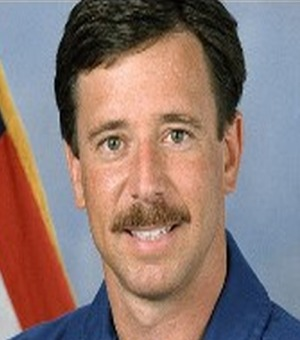
\includegraphics[width=1.8cm]{foto.jpg}};
\node[etapa, above=4pt of s1] {Escaneo};
\node[nota, below=3pt of s1] (n1) {12 s girando la cabeza;\\ángulo por la pose};

\node[foto] (s2) at (2.45, 0) {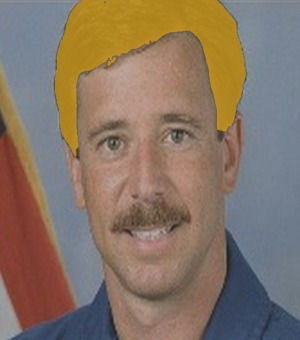
\includegraphics[width=1.8cm]{p_mascara.jpg}};
\node[etapa, above=4pt of s2] {Máscara};
\node[nota, below=3pt of s2] (n2) {segmentador, color\\del pelo y elipse};

\begin{scope}[shift={(5.15, -0.05)}, scale=0.52]
  \begin{scope}
    \clip[rotate=90] (-0.75, -3) rectangle (0.75, 3);
    \clip[rotate=30] (-0.904, -3) rectangle (0.904, 3);
    \clip[rotate=150] (-0.904, -3) rectangle (0.904, 3);
    \fill[blue!18] (-2, -2) rectangle (2, 2);
  \end{scope}
  \foreach \t/\c in {90/270, 30/30, 150/150} {
    \pgfmathsetmacro{\e}{sqrt((0.95*cos(\t))^2 + (0.75*sin(\t))^2)}
    \draw[blue, line width=0.5pt, dash pattern=on 2pt off 1.5pt, rotate=\t] (-\e, -1.55) -- (-\e, 1.55) (\e, -1.55) -- (\e, 1.55);
    \fill[ink, rotate=\c] (1.75, 0) -- ++(0.36, 0.2) -- ++(0, -0.4) -- cycle;
  }
  \draw[ink, line width=0.8pt, fill=yellow!35] (0, 0) ellipse (0.95 and 0.75);
\end{scope}
\node[etapa, anchor=south] at ($(5.15, 0 |- s2.north) + (0, 0.1)$) {Envolvente visual};
\node[nota] (n3) at (5.15, 0 |- n2) {cada vista limita dónde\\hay pelo; se intersecan};

\node[paso, text width=2.3cm, minimum height=1.9cm] (s4) at (7.95, 0) {%
  \textbf{Textura}\\[2pt]color de las vistas\\que mejor ven cada\\punto; dirección con\\el tensor de estructura};

\node[foto] (s5) at (10.55, 0) {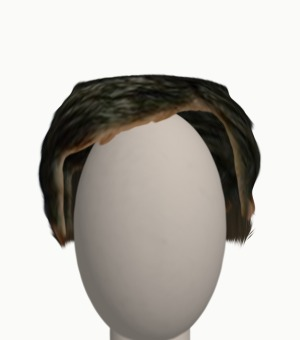
\includegraphics[width=1.8cm]{p_peluca.jpg}};
\node[etapa, above=4pt of s5] {Peluca};
\node[nota, below=3pt of s5] (n5) {gaussianas alargadas\\en la dirección del pelo};

\node[paso, text width=2.05cm, minimum height=1.9cm] (s6) at (13.0, 0) {%
  \textbf{Estudio}\\[2pt]color, largo y\\tijeras que cortan\\las gaussianas más\\cercanas};

\draw[flecha] (s1) -- (s2);
\draw[flecha] (s2) -- (4.0, 0);
\draw[flecha] (6.3, 0) -- (s4);
\draw[flecha] (s4) -- (s5);
\draw[flecha] (s5) -- (s6);

\coordinate (base) at ($(n2.south) + (0, -0.06)$);
\draw[llave=muted] (s1.west |- base) -- (s2.east |- base)
  node[midway, below=9pt, llavetexto=muted] {Captura};
\draw[llave=blue] (4.05, 0 |- base) -- (s4.east |- base)
  node[midway, below=9pt, llavetexto=blue] {Geometría y textura};
\draw[llave=red] (s5.west |- base) -- (s6.east |- base)
  node[midway, below=9pt, llavetexto=red] {Render y edición};

\end{tikzpicture}
\end{document}
